\documentclass[11pt, letterpaper, twoside]{article}
\usepackage[utf8]{inputenc}
\usepackage[T1]{fontenc}
\usepackage{fancyhdr}
\usepackage[margin=1in, include foot]{geometry}
\usepackage{ragged2e}
\usepackage[]{hyperref}
\usepackage{apacite}
\usepackage{setspace}
\usepackage{caption}
\usepackage{subcaption}
\usepackage{etoolbox}
\usepackage{graphicx}
\usepackage{amsmath, amssymb}
\usepackage{cleveref}
\usepackage{wrapfig}
\usepackage{afterpage}
\usepackage{floatrow}
\usepackage{tikz}
\usepackage{booktabs}
\usepackage{siunitx}
\usepackage{dcolumn}
\usepackage{pdflscape}


\setlength{\parindent}{0pt}
\floatsetup[table]{capposition=top}

\title{\singlespacing\textbf{\textit{Capitalisn't:} The Effects of Advertising on Audience Size}}


\author{Utsav Gandhi \thanks{Utsav Gandhi (utsav.gandhi@chicagobooth.edu), Stigler Center, Booth School of Business, University of Chicago}
    \and 
    Joshua Y. Levy \thanks{Joshua Y. Levy  (joshua.levy@chicagobooth.edu), Stigler Center, Booth School of Business, University of Chicago}}
\date{\today}

\onehalfspacing
\begin{document}
\begin{titlepage}
    \maketitle
    \thispagestyle{empty}
\end{titlepage}


\newpage
\pagenumbering{arabic}


% \begin{table}[!htbp] \centering 
    \caption{} 
    \label{} 
  \begin{tabular}{@{\extracolsep{5pt}} clccc} 
  \\[-1.8ex]\hline 
  \hline \\[-1.8ex] 
  Title & Release Date & Total Downloads & t14\_downloads \\ 
  \hline \\[-1.8ex] 
  The Capitalisn't Of Vaccines & 2020-09-24 & 13417 & 7872 \\ 
  The Right And Wrong Of MMT (Modern Monetary Theory) & 2020-10-08 & 18628 & 9241 \\ 
  Should We Lockdown Again? & 2020-10-22 & 13174 & 8080 \\ 
  What Is The Alternative To Friedman's Capitalism? & 2020-11-05 & 17398 & 8778 \\ 
  How The Supreme Court Influences Our Economy & 2020-11-19 & 12752 & 7645 \\ 
  Francis Fukuyama’s Proposal to Rein In Big Tech & 2020-12-03 & 14192 & 8085 \\ 
  How Do You Solve A Problem Like Student Debt? & 2020-12-17 & 14198 & 7740 \\ 
  Why Capitalism Needs Democracy & 2020-12-31 & 14516 & 8672 \\ 
  Microsoft 1998 vs Google 2020: Antitrust and Big Tech & 2021-01-14 & 15937 & 9338 \\ 
  Manufacturing Dissent With Matt Taibbi & 2021-01-28 & 16757 & 10088 \\ 
  GameStop, Robinhood And Our Troubling Obsession With Speculation & 2021-02-11 & 15004 & 9363 \\ 
  When the Profit Motive Kills With Anand Giridharadas & 2021-02-25 & 16426 & 9682 \\ 
  Why We Should Tax Digital Advertising With Paul Romer & 2021-03-11 & 13526 & 8233 \\ 
  Communisn’t: Crony Capitalism In China With David Barboza & 2021-03-25 & 14970 & 8725 \\ 
  The Power Of Access In Journalism And Academia With Kara Swisher & 2021-04-08 & 13110 & 8234 \\ 
  Is The Federal Reserve An "Engine of Inequality"? & 2021-04-22 & 14976 & 9095 \\ 
  Worried about Inflation? So is Fmr Central Banker Mervyn King & 2021-05-06 & 14589 & 9340 \\ 
  Who Will Regulate The Regulators: Stigler 50 Years Later & 2021-05-20 & 13706 & 8698 \\ 
  Why Do We Have High Prices But Stagnating Wages? & 2021-06-03 & 19182 & 11808 \\ 
  How The Elites Are Losing Control With Martin Gurri & 2021-06-17 & 18626 & 11429 \\ 
  The Price Of A Vaccine With Moderna CFO David Meline & 2021-07-01 & 15662 & 10067 \\ 
  The Engine No. 1 David vs Exxon Goliath With Chris James & 2021-07-15 & 16031 & 10369 \\ 
  The Promise Of Meritocracy With Adrian Wooldridge & 2021-07-29 & 16766 & 10827 \\ 
  The Cost of Meritocracy With Michael Sandel & 2021-08-12 & 20913 & 11892 \\ 
  The Breaking Point Of Democracy With Morton Schapiro and Gary Morson & 2021-08-27 & 17387 & 11158 \\ 
  The Smoke and Mirrors of ESG Investing with Tariq Fancy & 2021-09-09 & 18744 & 11396 \\ 
  Why Capitalism Isn't Without Democracy & 2021-09-23 & 17141 & 10961 \\ 
  Is Discrimination Still Causing The Gender Pay Gap With Claudia Goldin & 2021-10-07 & 18007 & 11897 \\ 
  Is Evergrande Really China’s Lehman Moment? & 2021-10-21 & 19369 & 13683 \\ 
  A Turning Point In The History Of Capitalism? & 2021-11-04 & 19134 & 13386 \\ 
  How Antitrust Failed Workers With Eric Posner & 2021-11-18 & 16528 & 11968 \\ 
  Is Woke Capitalism a Threat to Democracy? & 2021-12-02 & 17854 & 12888 \\ 
  The Political Polarization of Corporate America & 2021-12-16 & 16450 & 11849 \\ 
  Capitalism As A Contradiction With Yanis Varoufakis & 2022-01-06 & 17084 & 13254 \\ 
  Meritocracy: The Genetic Lottery with Kathryn Paige Harden & 2022-01-20 & 15701 & 13147 \\ 
  The Causes And Effects Of Today's Inflation, With Raghuram Rajan & 2022-02-03 & 17361 & 16579 \\ 
  The Private Equity Debate: Is it a Good Investment? & 2022-02-17 & 10414 & NA \\ 
  \hline \\[-1.8ex] 
  \end{tabular} 
  \end{table} 


\section{About \textit{Capitalisn't} and this investigation}
\textit{Capitalisn't} is a podcast hosted by Luigi Zingales and Bethany McLean about how ``the ways capitalism is --- or more often isn't --- working in our world today ... and what we can do to fix it.'' Released on a bi-weekly schedule, the podcast's reach has steadily grown since its inception in December 2017.\\

In order to expand the show's reach, the Stigler Center engaged in two advertising campaigns. What follows below is an anlaysis of the effectiveness of those campaigns in growing an audience for \textit{Capitalisn't}. We employ, ordinary-least squares (OLS), regression-discontinuity, and time-series regression methodologies in an effort to assess the effectiveness of those advertising campaigns.


\subsection{Advertising Campaigns}
In the course of advertising the podcast, the Stigler Center purchased two audio advertisements on journalism/economics-focussed media services. The first ad-spot was purchase from the Economist Media Group and a general call to action was played over Economist Radio podcasts between April 1st, 2021, and April 30th, 2021. At the price of \$12,000, over 30 days, advertisement reached 400,000 listeners. The second of the two audio ads, purchased from the Vox Media Group, aired over the \textit{Pivot} podcast, hosted by Kara Swisher and Scott Galloway. Between June 1st, 2021, and June 15th, 2021, this advertisement reached 455,000 listeners at the price of \$16,000. Additionally, the Stigler Center purchased an advertisement to run on LinkedIn, encouraging listeners to listen to a specific episode of the podcast: ``The Causes and Effects of Today's Inflation, with Raghuram Rajan,'' which originally aired on February 3rd, 2022.\\

The former audio-advertisements are henceforth referred to as ``general ads,'' in that the call to action is to listen to the podcast in general, and the latter LinkedIn advertisement is referred to as a ``specific ad'' because it encourages the viewer to listen to a specific episode.

\subsection{Data Summary}
This investigation primarily focusses on the effect of advertising on \textit{downloads} for \textit{Capitalisn't}.\footnote{Because mobile internet connectivity has improved considerably since the inception of podcasts, streaming has become a popular alternative to downloading episodes. However, because of the varying definitions of a ``stream'' among the varying distribution platforms for \textit{Capitalisn't} we focus on downloads, because it provides a readily-comparable, and therefore larger, sample for empirical analysis.} We collect the number of downloads of each podcast episode at the day-level temporal resolution from three distribution platforms: Simplecast, Spotify and Apple Podcasts. The number of day-downloads per episode is then summed over the three platforms so that each day-episode observation indicates the number of episode downloads made in that day over the three platforms. A table of episodes is available in Appendix A1.\\

We additionally collect various episode-level characteristics to be used as controls in econometric analysis. For each episode we collect:
\begin{itemize}
    \itemsep 0em
    \item whether the episode featured a guest;
    \item the Twitter and LinkedIn followers of those guests;
    \item whether the episode topic concerned a current event;
    \item a general category for the episode's topic (eg. COVID-19, economics, political economy, democracy, technology, ESG, etc.);
    \item whether the episode promoted a book;
    \item and whether at least one of the featured guests is a tenure-track academic. 
\end{itemize}
Table 1 includes a summary of these episode-level characteristics.


% Table created by stargazer v.5.2.3 by Marek Hlavac, Social Policy Institute. E-mail: marek.hlavac at gmail.com
% Date and time: Fri, Mar 25, 2022 - 11:01:09 AM
\begin{table}[!htbp] \centering 
  \caption{Episode-level Charateristics: Summary Statistics} 
  \label{} 
\begin{tabular}{@{\extracolsep{5pt}}lccccc} 
\\[-1.8ex]\hline 
\hline \\[-1.8ex] 
Statistic & \multicolumn{1}{c}{N} & \multicolumn{1}{c}{Mean} & \multicolumn{1}{c}{St. Dev.} & \multicolumn{1}{c}{Min} & \multicolumn{1}{c}{Max} \\ 
\hline \\[-1.8ex] 
Features guest & 37 & 0.919 & 0.277 & 0 & 1 \\ 
Features multiple guests & 37 & 0.135 & 0.347 & 0 & 1 \\ 
Current event ep. & 37 & 0.216 & 0.417 & 0 & 1 \\ 
Book promo ep. & 37 & 0.189 & 0.397 & 0 & 1 \\ 
Tenured guest & 37 & 0.676 & 0.475 & 0 & 1 \\ 
Guest(s) Twitter followers & 37 & 141,307.200 & 323,350.200 & 0 & 1,400,000 \\ 
Guest(s) LinkedIn followers & 37 & 34,343.080 & 197,844.300 & 0 & 1,205,108 \\ 
\hline \\[-1.8ex] 
\end{tabular} 
\end{table} 


\subsection{Exploratory data visualization}
Figure 1 displays two plots illustrating the primary trend explaining the growth of the podcast: time. Panel (a) plots an episodes cumulative downloads over time (days since release). Each line represents a different episode. There are three phenomenon of note. First, episodes, see a large share of their downloads occur in the first days following release. Secondly, most episodes have a ``long tail'' of downloads that continue to take place well after the initial release. Note that the slope of each line positive even for a long period following release. Finally, over time (as indicated by the colors of each line) the initial period following release sees more downloads than prior episodes. This ``upwards'' bending of the curve indicates a strong time-fixed effect of the podcast gaining popularity over time. Panel (b) plots the same data as Panel (a) but with a logarithmic horizontal axis. This more clearly illustrates the second and third phenomena identified in Panel (a). The greater-than-1 linear-log relationship indicates that episodes continue to be downloaded over time. Additionally, note that over time (as the lines become lighter in color), the vertical intercept rises --- indicating greater first-day downloads (the growing popularity of the podcast over time). These panels motivate the naive regression analysis presented in Section INSERT NUMBER HERE.\\


% Figure 1 
\begin{figure}[h]
    \centering
    \begin{subfigure}[h]{0.49\textwidth}
        \centering
        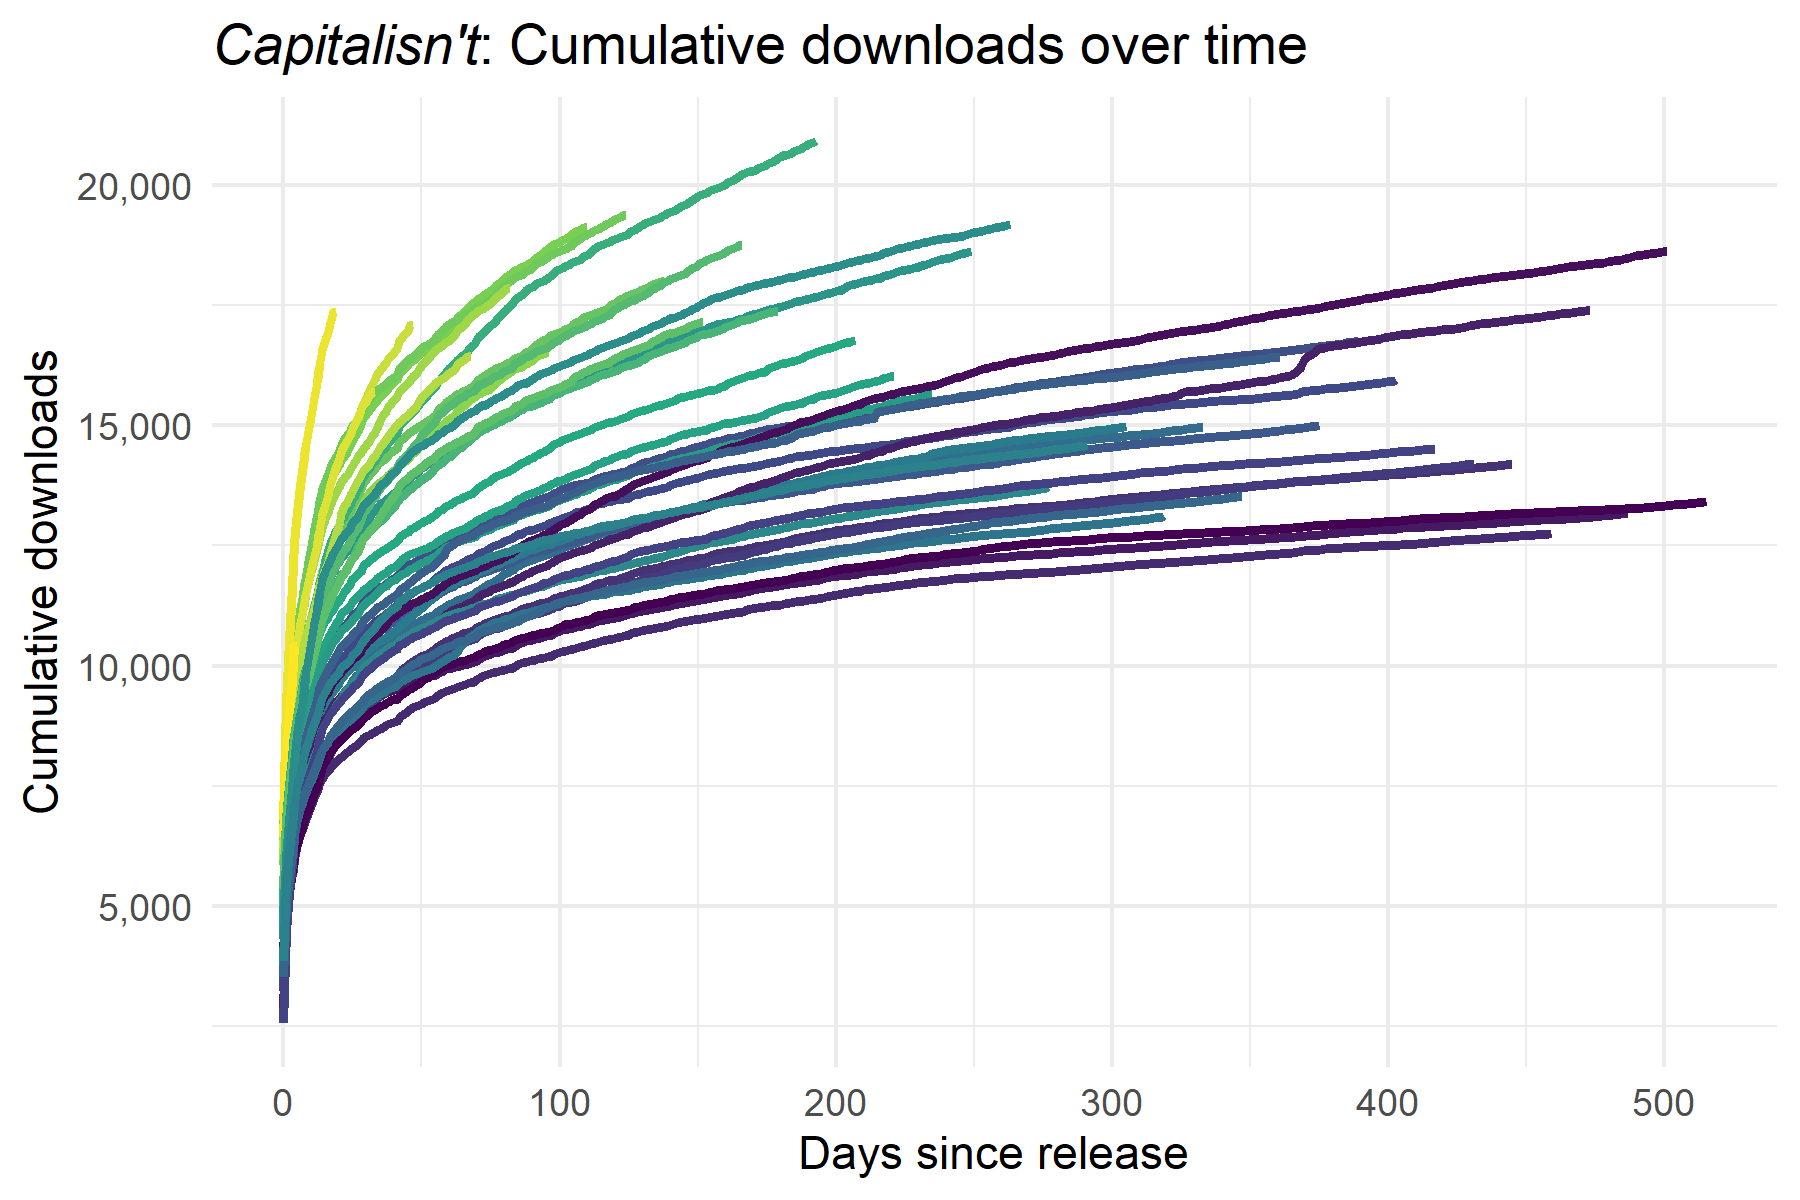
\includegraphics[width=\textwidth]{cumulative_downloads_since_release.png}
        \caption{}
    \end{subfigure}
    \hfill
    \begin{subfigure}[h]{0.49\textwidth}
        \centering
        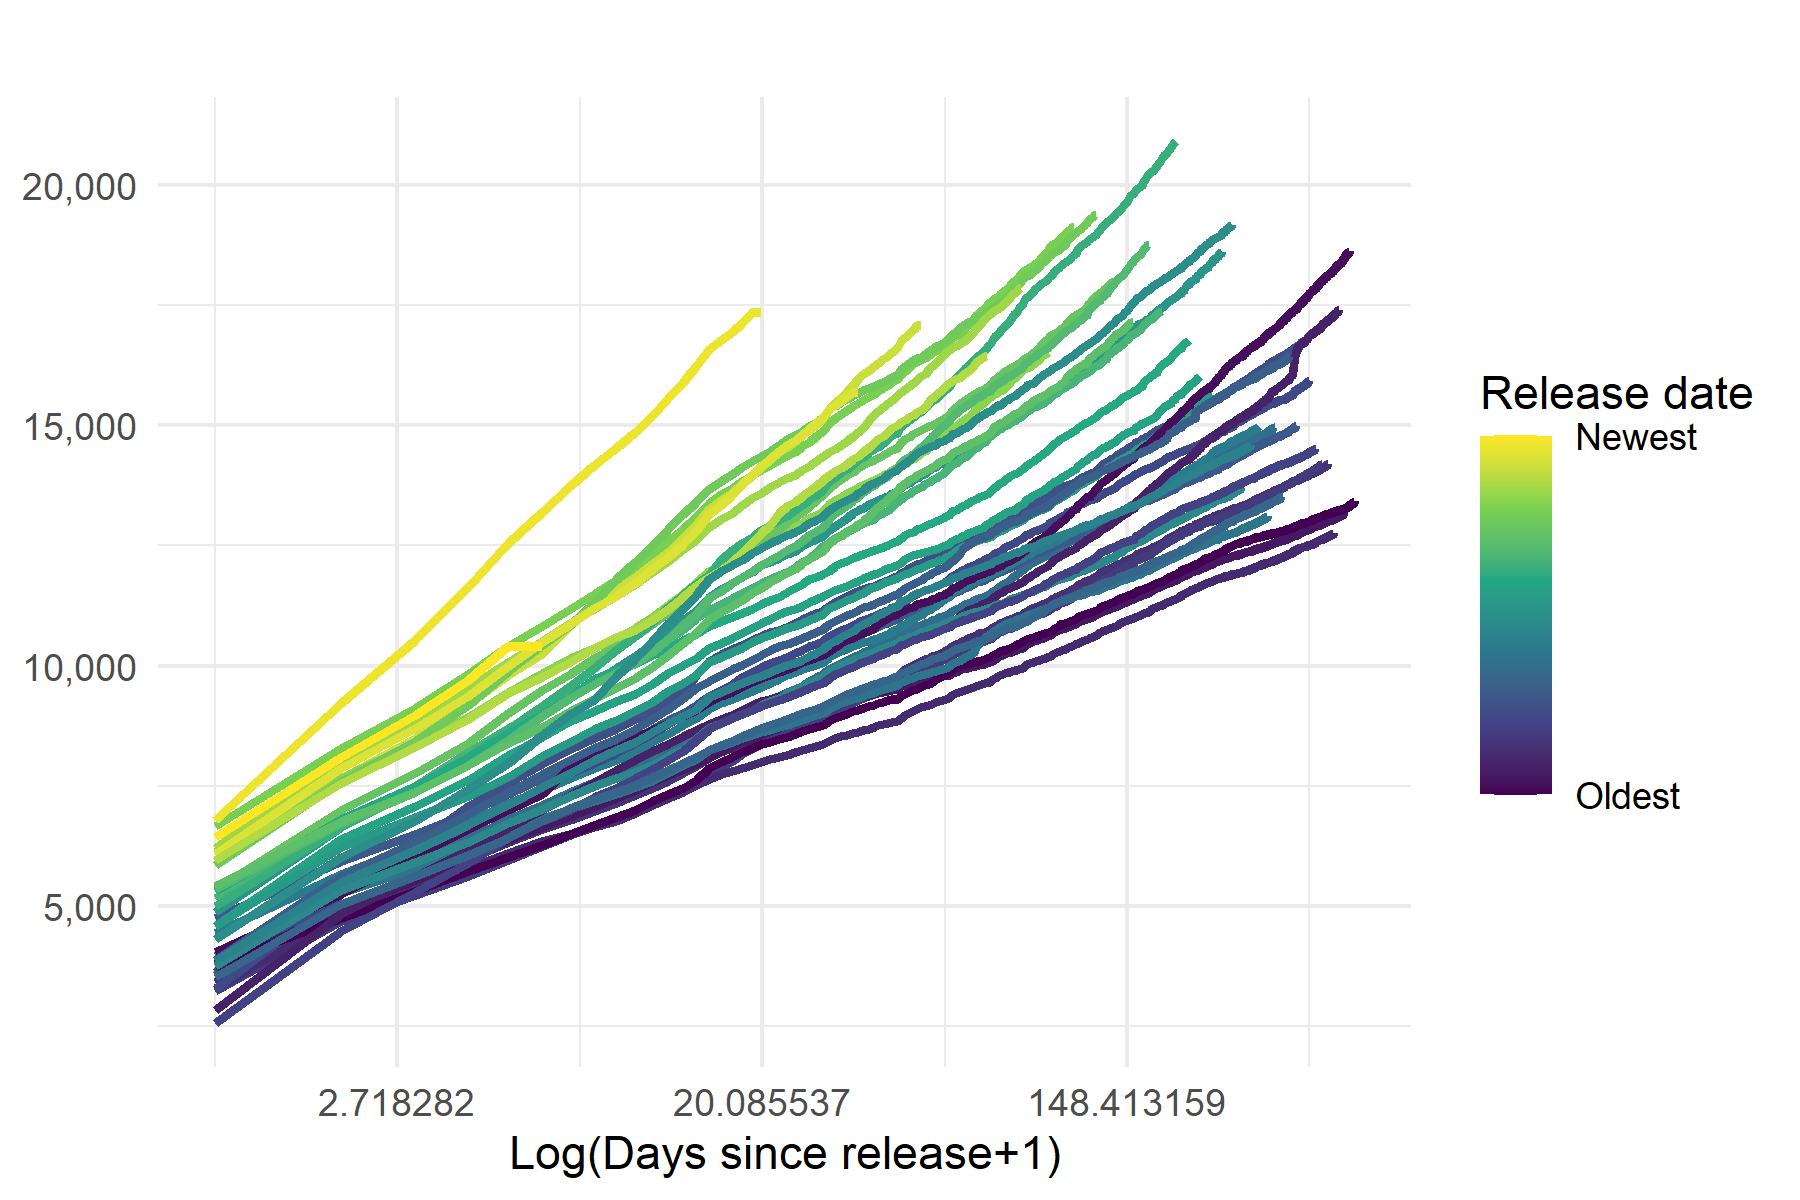
\includegraphics[width=\textwidth]{cumulative_downloads_since_release_log.png}
        \caption{}
    \end{subfigure}
    \caption{Cumulative downloads over time}
\end{figure}

Figure 2 presents two plots that show the evolution of the podcast over time. Panel (a) shows the aggregate number of podcast downloads across all podcasts every day since the release of the first episode for which we have an observation (``The Capitalisn't of Vaccines,'' released on September 24th, 2020.) There are three observations of interest. First, the bi-weekly release schedule of the podcast is evident in the ``spiky'' periodic peaks and valleys. Second, the peaks rise over time. This is indicative of rising first-day downloads (though it also includes downloads of back-catalog episodes on the day of a new episode's release). Finally, note that over time, the ``troughs'' rise. This indicates either that the there are more back-catalog downloads between episodes, or listeners downloading the most recent episode increasingly late (not immediately following release), or some combination of both. Panel (b) shows the cumulative downloads of all episodes following their release.\footnote{The opacity of each line decreases over time so as to make the trace of each new-episode relatively easier to identify against the background catalog.} The rising number of first-day downloads is evident here as the first-value plotted for each episode tends upwards over time. Additionally, note that more recent episodes see the coefficient leading the logarithmic function grow over time. That is, newer episodes not only see more first-day downloads, but they also see more second-, third-, and fourth-day (etc.) downloads as well.\footnote{The relationship between the values plotted in Panels (a) and (b) is as follows. The value plotted in Panel (a) at time $t$, denoted as $v_{at}$ is equal to the sum of all the one-day differences for all episodes, $i$ released prior to time $t$. $$v_{at} = \sum_{i \in \mathbb{B}} v_{it} - v_{it-1} \quad \text{where} \quad \mathbb{B}= \{i: i_{release} \leq t\}$$}\\

% Figure 2
\begin{landscape}
    \thispagestyle{empty}
    \begin{figure}[h]
        \centering
        \begin{subfigure}[h]{\textwidth}
            \centering
            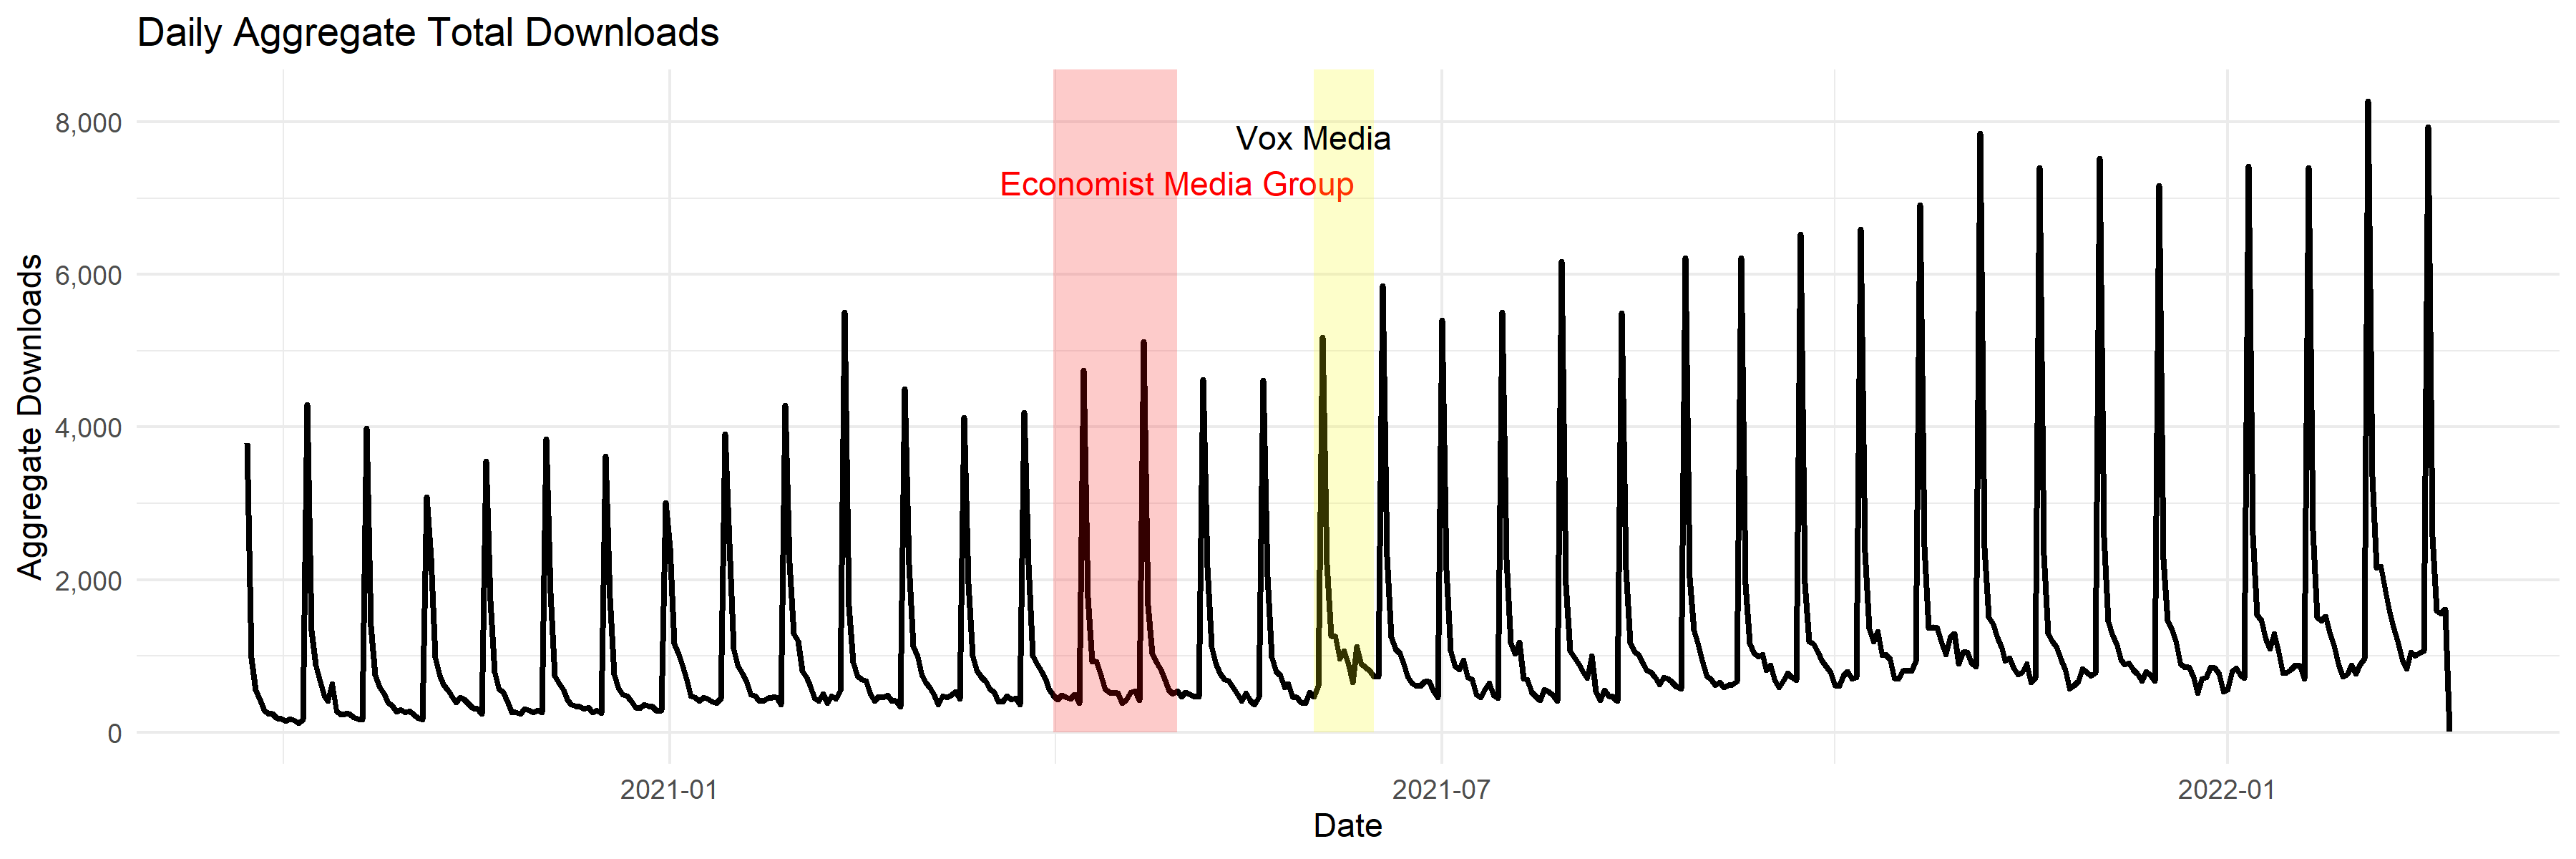
\includegraphics[width=\textwidth]{daily_aggregate_download.png}
            \caption{}
        \end{subfigure}
        \vspace{1em}
        \begin{subfigure}[h]{\textwidth}
            \centering
            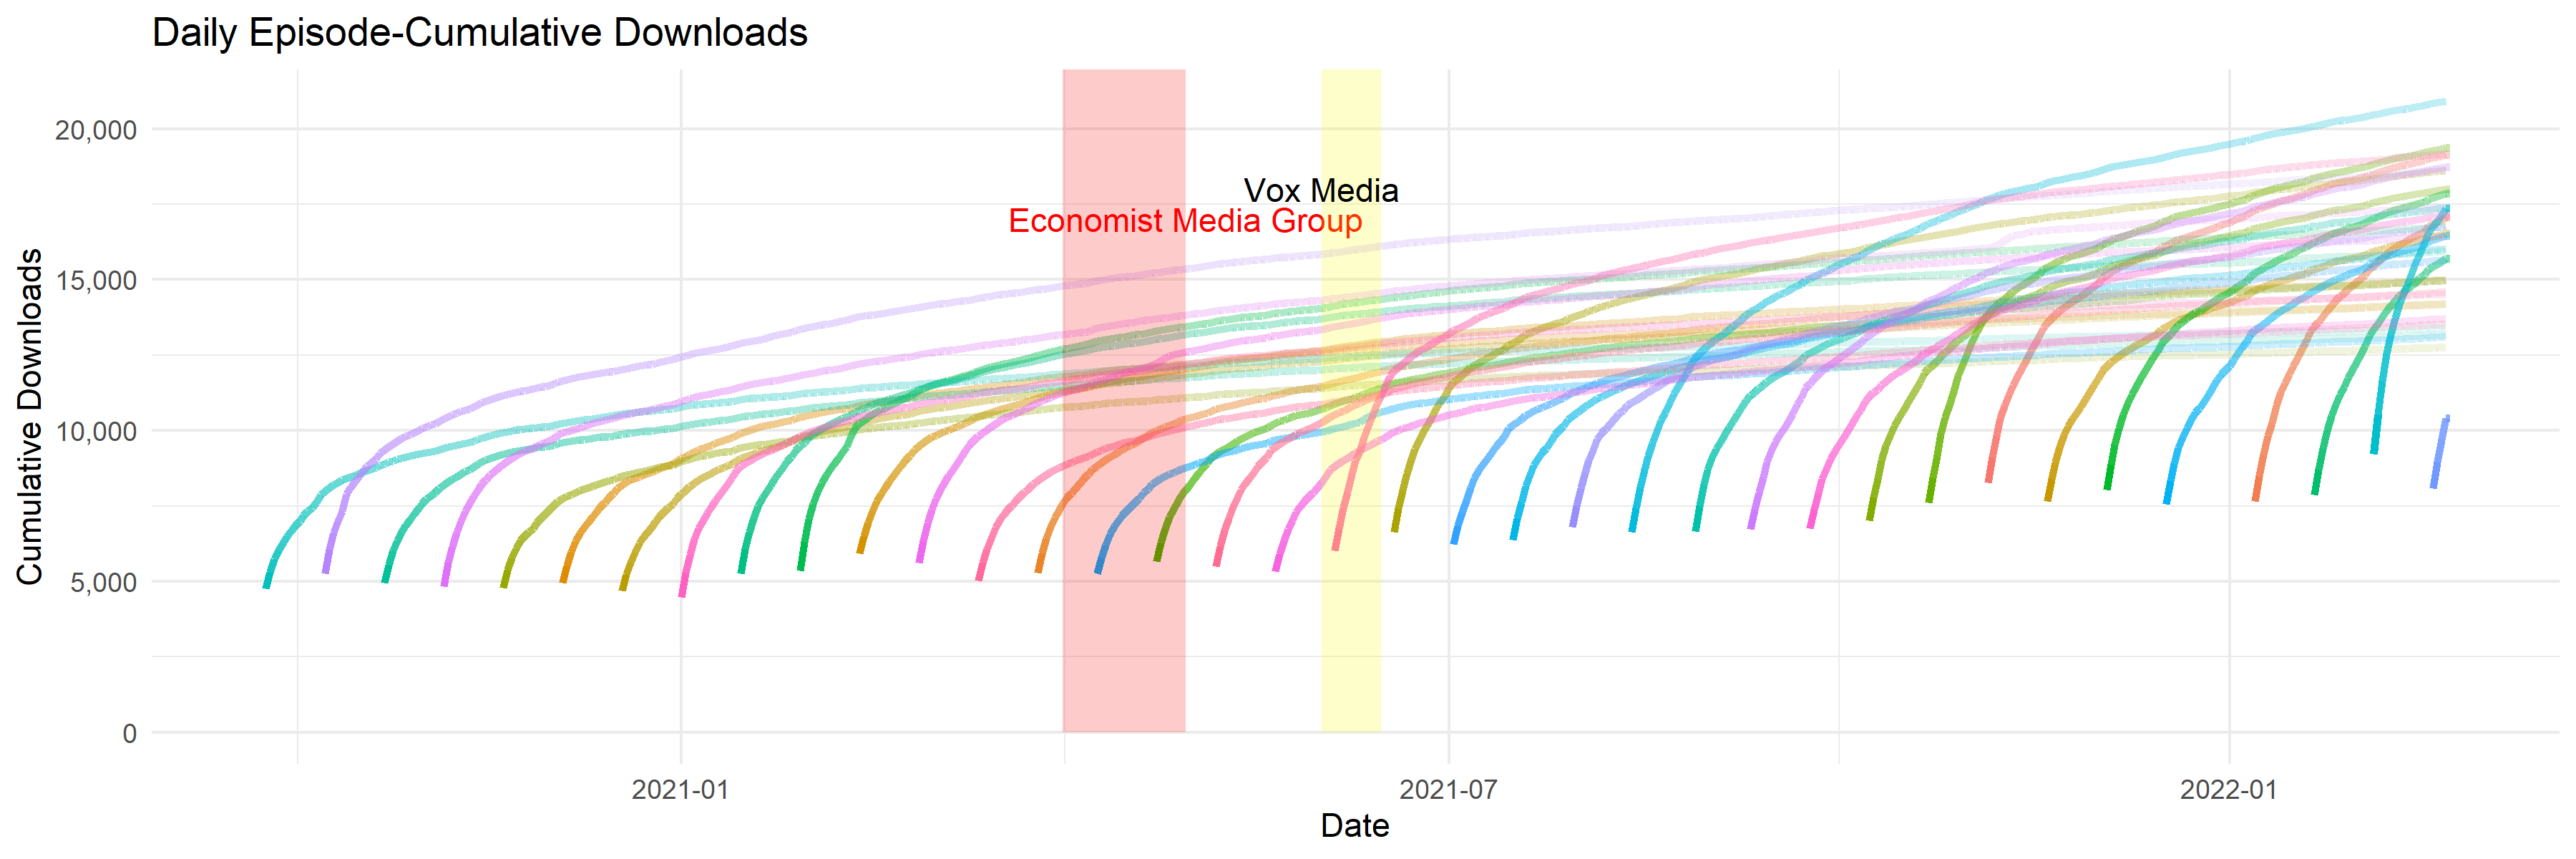
\includegraphics[width=\textwidth]{daily_cumulative_download.png}
            \caption{}
        \end{subfigure}
        \caption{Podcast downloads over time}
    \end{figure}
\end{landscape}


In both figures, the period shaded in red represents the period during which the Economist Media Group advertisement was airing (April 1st, 2021 to April 30th, 2021). The period shaded in yellow represents the period during which the Vox Media Group advertisement was airing (June 1st, 2021 to June 15th, 2021.) Of particular interest is the relatively ``high trough'' following the release of the episode ``Why Do We Have High Prices But Stagnating Wages?'' released on June 3rd, 2021. This episode appears to have, itself, performed very well, as demonstrated in panel (b) with a large increase in cumulative downloads between June 3rd and June 4th. This is doubly interesting because it takes place during the Vox general ad period. These panels motivate the regression analysis presented in Section INSERT NUMBER HERE.





\section{Empirical Analysis}
\subsection{Naive Estimates}
We begin with naive estimation of the covariates that predict an episode's performance. Table 2 contains regression estimates for the cumulative downloads of an episode at $t=14$ days after release.\footnote{We choose to initially estimate cumulative downloads at $t=14$ because this is the last day for which download-data is available before the release of the next episode. That is, this is the last point at which we are able to estimate the performance of an episode without having to control for the characteristics of subsequent episodes.} The ``Trailing Avg.'' explanatory variable is computed as the average of the previous five episodes' cumulative downloads 14 days after each of their releases.\footnote{For the first four episodes in the sample, instead of using a five-episode trailing average, a one-, two-, three-, and four-episode trailing average is used. These observations are omitted from the sample in model (2).} We use this measure to account for the growth of the podcast over time as the small sample of episodes would make time fixed effects inappropriate due to over-fitting. ``General Ad,'' ``Specific Ad,'' ``Book Promo,'' and ``Tenure(d) Guest'' are all dichotomous variables. The first two advertisement-related variables are coded as 1 if an advertisement of the given type was in progress during the air-date of the episode. ``Book Promo'' is coded as 1 if the episode promotes a book. ``Tenure(d) Guest'' is coded as 1 if at least one of the guests on an episode is a tenure-track faculty member at a university. Heteroskedastic-robust errors are presented in parentheses.\\

% Table 2 : Naive OLS reg results

% Table created by stargazer v.5.2.3 by Marek Hlavac, Social Policy Institute. E-mail: marek.hlavac at gmail.com
% Date and time: Mon, Mar 28, 2022 - 8:48:35 PM
\begin{table}[h] \centering 
  \caption{Naive OLS estimates} 
  \label{} 
\small 
\begin{tabular}{@{\extracolsep{5pt}}lccccc} 
\\[-1.8ex]\hline 
\hline \\[-1.8ex] 
 & \multicolumn{5}{c}{\textit{Dependent variable:}} \\ 
\cline{2-6} 
\\[-1.8ex] & \multicolumn{5}{c}{Cumulative downloads ($t=14$)} \\ 
 & Baseline & Trimmed & Ads & Book Promo & Tenure \\ 
\\[-1.8ex] & (1) & (2) & (3) & (4) & (5)\\ 
\hline \\[-1.8ex] 
 Trailing Avg. & 0.978$^{***}$ & 0.957$^{***}$ & 1.007$^{***}$ & 0.957$^{***}$ & 1.008$^{***}$ \\ 
  & (0.112) & (0.123) & (0.108) & (0.129) & (0.108) \\ 
  Twitter Followers & $-$0.0004 & $-$0.0004 & 0.0003 & $-$0.0005 & 0.0003 \\ 
  & (0.001) & (0.001) & (0.001) & (0.001) & (0.001) \\ 
  LinkedIn Followers & 0.003$^{***}$ & 0.003$^{***}$ & $-$0.155 & 0.003$^{***}$ & $-$0.156 \\ 
  & (0.001) & (0.001) & (0.119) & (0.001) & (0.126) \\ 
  General Ad$^{\dag}$  &  &  & 967.938 &  & 968.017 \\ 
  &  &  & (1,032.957) &  & (1,054.355) \\ 
  Specific Ad$^{\dag}$ &  &  & 190,208.100 &  & 191,251.500 \\ 
  &  &  & (143,547.300) &  & (152,350.900) \\ 
  Book Promo$^{\dag}$ &  &  &  & 210.517 &  \\ 
  &  &  &  & (421.231) &  \\ 
  Tenure(d) Guest$^{\dag}$ &  &  &  &  & $-$10.008 \\ 
  &  &  &  &  & (441.884) \\ 
  Constant & 691.356 & 935.142 & 415.380 & 869.804 & 415.951 \\ 
  & (1,129.228) & (1,271.373) & (1,077.631) & (1,248.578) & (1,103.356) \\ 
 \hline \\[-1.8ex] 
Observations & 34 & 30 & 34 & 34 & 34 \\ 
R$^{2}$ & 0.790 & 0.782 & 0.809 & 0.791 & 0.809 \\ 
Adjusted R$^{2}$ & 0.769 & 0.756 & 0.775 & 0.762 & 0.766 \\ 
\hline 
\hline \\[-1.8ex] 
\textit{Note:}  & \multicolumn{5}{r}{$^{*}$p$<$0.1; $^{**}$p$<$0.05; $^{***}$p$<$0.01} \\ 
 & \multicolumn{5}{r}{$^{\dag}$ inidcates variable is dichotomous} \\ 
\end{tabular} 
\end{table} 


In this naive setting, model (3) is our preferred specification. Note that across this suite of regressions, only the ``trailing average'' variable is regularly statistically significant. However, in all but models (3) and (5), the coefficient on this regressor is slightly below 1. That is, these regressions estimate that for each download that the previous five episodes received by the fourteenth day after their release, the episode of interest will have only received between 0.957 and 0.978 downloads. This implies a downward trajectory for the performance of the podcast generally, which is incongruent with even a prima facie analysis of the podcast's long-run performance. For this reason, the greater-than-one coefficients on ``trailing average'' in models (3) and (5) are preferable. Secondly, consider how in models (1), (2) and (4), ``LinkedIn Followers'' appears to have a positive and statistically significant (if small) effect on episode downloads. This significance disappears however, if the ``specific ad'' regressor is also included in the regression. Closer inspection of the underlying data reveals that this is due to an outlier-guest, Raghuram Rajan, who has a particularly large LinkedIn following. Moreover, because the ``specific ad'' dichotomous variable is effectively a fixed-effect variable for the episode on which Rajan featured, all of the effect of Rajan's LinkedIn following is completely absorbed, leaving the ``LinkedIn followers'' regressor with no explanatory power. Comparing models (3) and (5), we prefer model (3) because they produce similar coefficient estimates but model (3) does so with fewer regressors. This is preferable in light of the very small sample size available.\\

Notably, in these specification, advertising appears to have no statistically significant effect on the performance of an episode as measured by cumulative downloads 14 days following release. We further investigate the effects of advertising using other framings of performance. 

\subsection{Effects of Advertising}
Table 3 contains the results corresponding to models that are motivated by Figure 1(b). That is, cumulative downloads at day $t$ after release is a largely logarithmic function of days since release.\footnote{In these regressions, the measure of ``days since release'' has been transformed so that the day of release, $t_{release}=1$. This transformation is used to make interpretation of the constant (note the high degree of significance across all specifications) and coefficient (for $t$ on the interval $[0,1)$) easier to interpret. } Heteroskedastic-robust standard errors are presented in parentheses. The baseline regression model (1) includes no controls and simply attempts to confirm the logarithmic relationship between time since release and cumulative downloads. Model (2) includes dichotomous variables for whether the observation of interest occurred during a general- or specific-ad period. Though the negative coefficient defies expectations, see below for further exploration of why sample selection might explain this result.\\

Because the ``specific ad'' regressor effectively serves as a fixed-effect for the Rajan episode, it is omitted in the remainder of specifications. Model (3) explores the effects of the general-ad campaigns more closely. ``General ad'' is coded as before, and ``between general ads'' is coded as 1 if the date for the observation of interest falls between May 1st, 2021 and May 31st, 2021, the interval between the Economist and Vox advertisements. ``Post-General Ads'' is coded as 1 if the observation of interest is dated after June 15th, 2021. Unlike in model (2), the signs on these coefficients are positive, as would be expected for a successful advertising campaign. However, when taken together, they imply a counter-intuitive relationship. One would expect that the advertisements drive the most additional downloads while they are being aired and while they are most salient to potential downloaders who hear the ad. However, the increasing magnitude of coefficients imply exactly the opposite: that although advertisements encourage downloads while they are being aired, they are even more effective at encouraging downloads after they have stopped airing.\\ 

%Figure 3
\begin{figure}[h]
    \centering    
    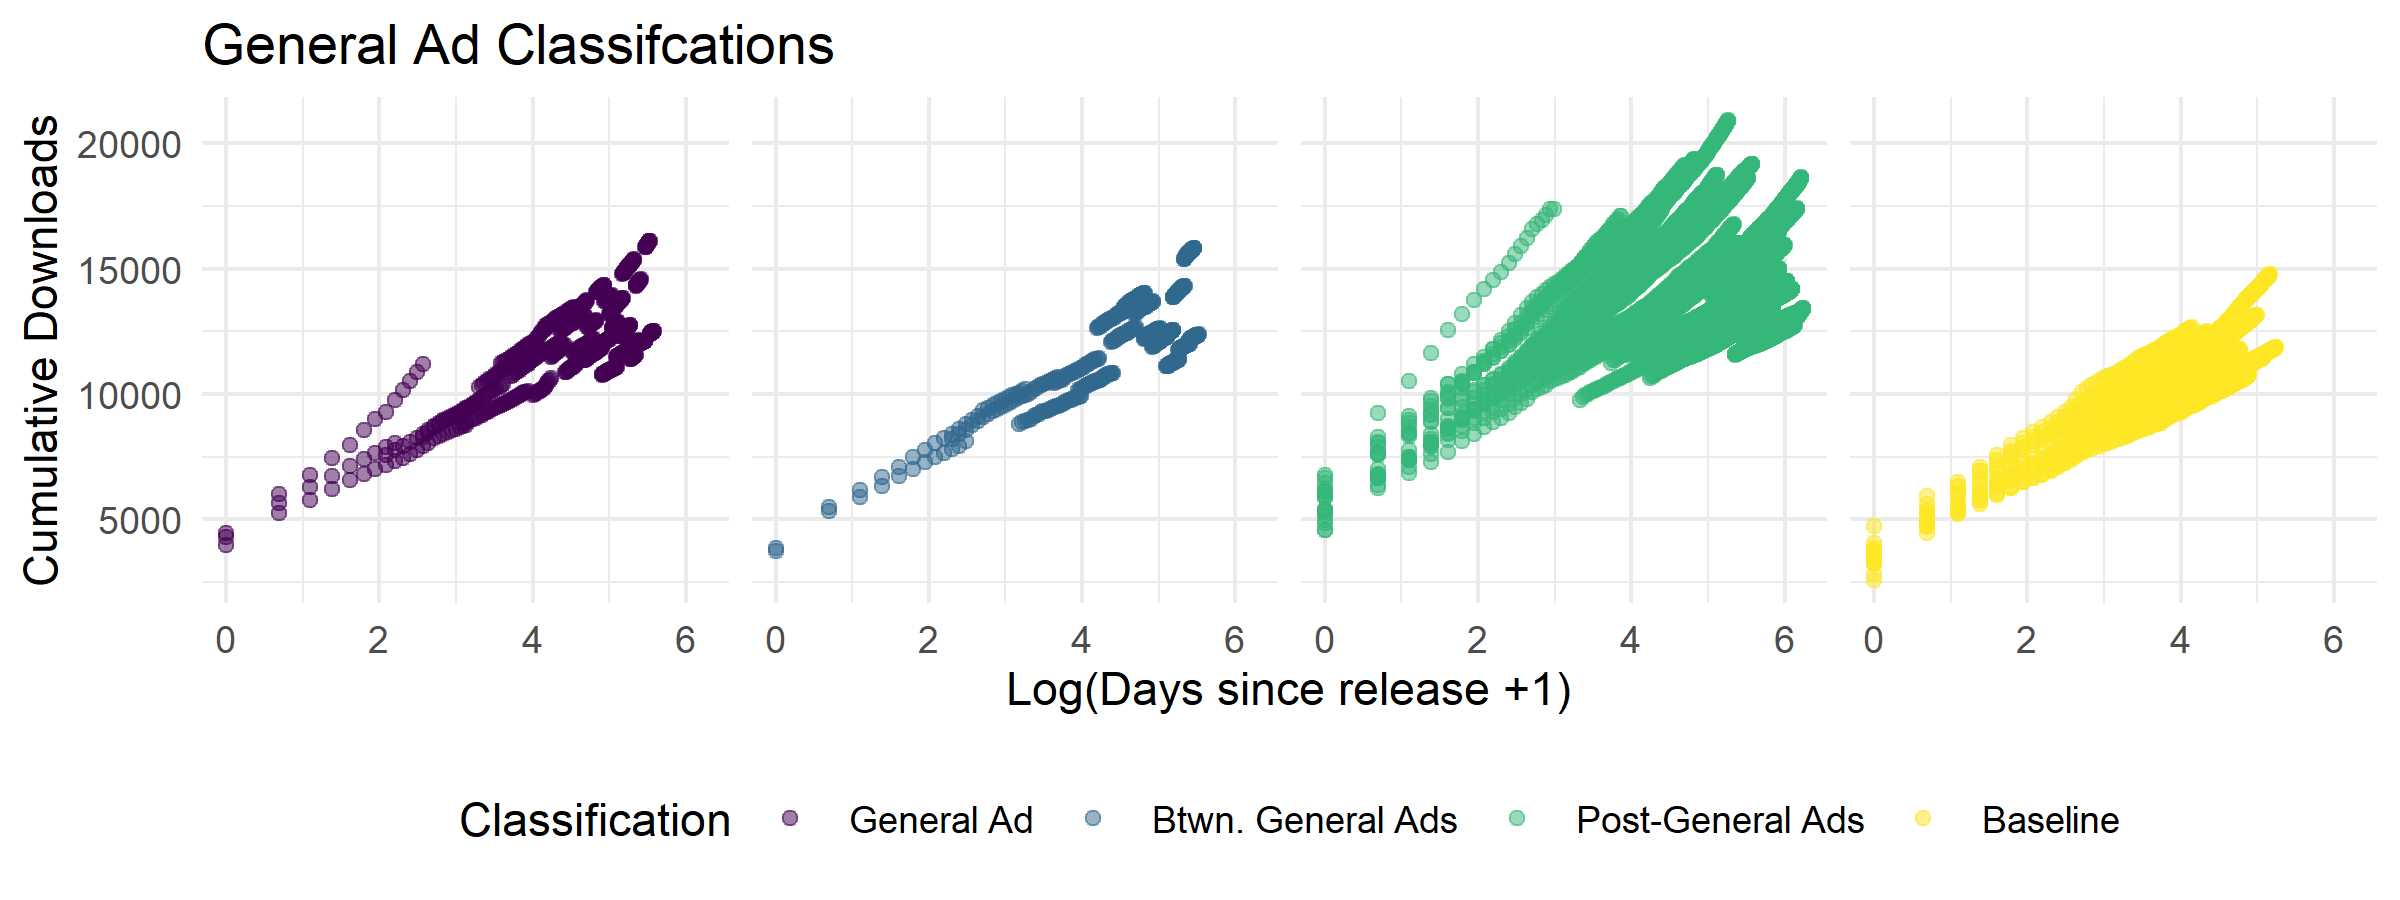
\includegraphics[width=\textwidth]{general_ad_class_plot.png}
    \caption{Breakdown of temporal binary regressors}
\end{figure}


This is likely due to the construction of the sample used in this specification. Note that episodes that are released after the advertising period ends are also the most recent episodes, i.e. those that are likely to receive the most first-day downloads by virtue of the podcast's secular growth over time. As is clear in Figure 3, this causes the intercept for the sub-group (post-general in green) to rise, increasing the magnitude of the corresponding coefficient on the binary regressor.\\

To resolve this challenge, we restrict the sample in model (4) --- our preferred model --- to include only episodes that were released prior to the general-ad campaigns. That is, we would hypothesize that those episodes that are ``treated'' (are already in the back-catalog prior ) should see a deviation from their download trajectory after the ad campaigns. In short, we should see an increase in the rate that episodes accrue cumulative downloads \textit{following} advertisement. This is captured by the interaction term, ``$\log(\text{Days since release})\times$Post-General'' in model (4).\footnote{In this specification, ``post-general'' only appears as an interaction, and not alone as binary regressor. We omit the binary regressor because, if included, its coefficient implies the increase in cumulative downloads increases step-wise from the first day of release if the episode is treated. This, however, is not the case. We would theorize that there should be a step-wise increase in downloads from the day of first treatment, which is different for each episode as this regression framework regresses on a normalized days-since-release measure.} Note the positive and highly statistically significant coefficient on this interaction term. Despite the strong linear-log relationship, we are hesitant to extrapolate the regression results for the purposes of causal inference or interpretation. That is, these results indicate that the rate of cumulative downloads increases by 156 downloads per unit increase in $\log(\text{Days since release})$. This does \textit{not} imply a 10\% increase \textit{relative} to a counterfactual. Rather, the statistical significance of the interaction term implies the existence of ``kink'' that suggests that, within episodes, download behavior differs prior to and following the advertising campaign.\footnote{As it corresponds to the panels in Figure 1, the advertising campaign can be thought of as bending any treated episode's curve ``upwards''.}\\

The specification detailed in model (5) is similar to that in model (4). However, the interaction term regressor is positive if the date of the observation is any time after the first date of the first general advertisement campaign --- April 1st, 2021 (and zero otherwise). We construct this version of ``Any General'' because the prior definition used in model (4) only treats observations as treated if it takes place after the ad campaign \textit{ends}. It stands to reason that the ad campaign would have a smaller estimated effect on an episode's download trajectory if the period during which the advertisement campaign is in progress is not included. That is, we might think that the advertisements drive the most additional downloads while the advertisements are airing. So, ``Any General'' is coded as 1 even if an episode is only ``partially treated'' at the date of observation --- for instance, in the case when an observation takes place after the Economist ad has run but before the Vox ad campaign has begun. As expected, the coefficient on this term, which remains highly statistically significant, is slightly larger than the corresponding coefficient in model (4). However, the coefficient on the primary temporal trend, ``$\log(\text{Days since release})$'' is smaller by almost as much as the coefficient on the interaction term is larger.\footnote{This is the extent to which we attempt to conduct any kind of ``placebo'' testing in this framework. We stop here because assuming we cannot define advertising exposure as an arbitrary threshold in the usual regression-discontinuity (RDD) sense. RDD assumes that arbitrary assignment is pseudo-random with respect to unobservables and that by running a ``placebo'' regression with a different assignment threshold should undermine the results of the regression using the true threshold. We have two options: 1) move the placebo advertisement dates forward (later) considerably; or 2) move the placebo advertisement dates backwards (earlier) considerably. We do not do either of these because in this framework, the normalized days-since-release regressor complicates the assignment of a placebo. Because treatment takes place over a window of time, we would have to move the placebo by at least width of the window.} This result confirms the idea that advertising is most effective around the time of the advertising campaign even if the advertising ``treatment'' campaign is not complete.\\

\begin{landscape}
    \thispagestyle{empty}
    
% Table created by stargazer v.5.2.3 by Marek Hlavac, Social Policy Institute. E-mail: marek.hlavac at gmail.com
% Date and time: Tue, Mar 29, 2022 - 10:12:40 PM
\begin{table}[h] \centering 
  \caption{Cumulative Downloads vs Log(days since release)} 
  \label{} 
\small 
\begin{tabular}{@{\extracolsep{5pt}}lccccc} 
\\[-1.8ex]\hline 
\hline \\[-1.8ex] 
 & \multicolumn{5}{c}{\textit{Dependent variable:}} \\ 
\cline{2-6} 
\\[-1.8ex] & \multicolumn{5}{c}{Cumulative downloads} \\ 
 & Baseline & Ad Campaigns & General Ads & Interaction & Interaction (fuzzy) \\ 
\\[-1.8ex] & (1) & (2) & (3) & (4) & (5)\\ 
\hline \\[-1.8ex] 
 $\log{(\text{Days since release})}$ & 1,387.192$^{***}$ & 1,382.386$^{***}$ & 992.294$^{***}$ & 1,541.081$^{***}$ & 1,509.464$^{***}$ \\ 
  & (18.777) & (18.568) & (20.625) & (20.536) & (20.619) \\ 
  & & & & & \\ 
 General Ad $^{\dag}$ &  & $-$1,248.214$^{***}$ & 884.710$^{***}$ &  &  \\ 
  &  & (47.616) & (56.291) &  &  \\ 
  & & & & & \\ 
 Specific Ad $^{\dag}$ &  & 4,468.642$^{***}$ &  &  &  \\ 
  &  & (404.967) &  &  &  \\ 
  & & & & & \\ 
 Btwn. General Ads $^{\dag}$ &  &  & 922.134$^{***}$ &  &  \\ 
  &  &  & (64.268) &  &  \\ 
  & & & & & \\ 
 Post-General Ads $^{\dag}$ &  &  & 2,818.333$^{***}$ &  &  \\ 
  &  &  & (45.784) &  &  \\ 
  & & & & & \\ 
 $\log{(\text{Days since release})} \times$ Post-General &  &  &  & 156.945$^{***}$ &  \\ 
  &  &  &  & (8.156) &  \\ 
  & & & & & \\ 
 $\log{(\text{Days since release})} \times$ Any General &  &  &  &  & 199.518$^{***}$ \\ 
  &  &  &  &  & (9.008) \\ 
  & & & & & \\ 
 Constant & 6,809.528$^{***}$ & 6,917.401$^{***}$ & 6,523.706$^{***}$ & 4,731.234$^{***}$ & 4,586.110$^{***}$ \\ 
  & (94.364) & (94.249) & (86.233) & (82.708) & (76.690) \\ 
  & & & & & \\ 
\hline \\[-1.8ex] 
Observations & 9,752 & 9,752 & 9,752 & 7,410 & 7,410 \\ 
R$^{2}$ & 0.340 & 0.363 & 0.492 & 0.618 & 0.616 \\ 
Adjusted R$^{2}$ & 0.340 & 0.363 & 0.492 & 0.618 & 0.616 \\ 
\hline 
\hline \\[-1.8ex] 
\textit{Note:}  & \multicolumn{5}{r}{$^{*}$p$<$0.1; $^{**}$p$<$0.05; $^{***}$p$<$0.01} \\ 
 & \multicolumn{5}{r}{$^{\dag}$ inidcates variable is dichotomous} \\ 
\end{tabular} 
\end{table} 
 
\end{landscape}




\section{Quantification}






\end{document}